\documentclass[12pt,a4paper]{article}

%========================= Pacotes Básicos =====================================
\usepackage[utf8]{inputenc}             % Codificação UTF-8
\usepackage[greek,english,portuguese]{babel} % Idiomas suportados
\usepackage{alphabeta}                 % Suporte para caracteres gregos
\usepackage{amssymb, amsmath}          % Matemática
\usepackage{subcaption}                % Subfiguras

%========================= Configuração de Gráficos ============================
\usepackage[pdftex]{graphicx}          % Inclusão de imagens
\usepackage[top=1in, bottom=1in, left=1in, right=1in]{geometry} % Margens

%========================= Aparência do Texto ==================================
\linespread{1.06}                      % Espaçamento entre linhas
\setlength{\parskip}{8pt plus2pt minus2pt} % Espaçamento entre parágrafos
\widowpenalty 10000                    % Evita linhas órfãs
\clubpenalty 10000                     % Evita linhas viúvas

%========================= Novos Comandos ======================================
\newcommand{\eat}[1]{}                 % Comando para ignorar texto
\newcommand{\HRule}{\rule{\linewidth}{0.5mm}} % Linha horizontal customizada

%========================= Pacotes Extras ======================================
\usepackage[official]{eurosym}         % Suporte ao símbolo do euro (€)
\usepackage{enumitem}                  % Listas personalizadas
\setlist{nolistsep,noitemsep}          % Configuração padrão para listas
\usepackage[hidelinks]{hyperref}       % Links sem formatação
\usepackage{lipsum}                    % Texto de preenchimento

% ESSE IMPORTE PRO BIBTEX TEM QUE ESTAR NO FINAL DO PREAMBULO
% SE TIRAR DAQUI NAO VAI FUNCIONAR
\usepackage[alf]{abntex2cite}	% Citações padrão ABNT

%========================= Documento ===========================================
\begin{document}

%========================= Página de Título ====================================
\begin{titlepage}
\begin{center}

~\\[1.5cm]

\includegraphics[width=0.45\textwidth]{UFMG.png}~\\[1.5cm]

% Título
\HRule \\[0.4cm]
{ \LARGE 
  \textbf{Laboratório de Sistemas 3}\\[0.4cm]
  \emph{Relatório Kanban}\\[0.4cm]
  \emph{Engenharia de Sistemas}\\[0.3cm]
  \emph{Grupo C}\\[0.3cm]
}
\HRule \\[1.5cm]

% Autor
{ \large
  Henrique Perim {\|} \texttt{2019042554} \\[0.1cm]
}

\vfill

\textsc{\large Departamento de Engenharia Elétrica da Universidade Federal de Minas Gerais}\\[0.4cm]

% Data
{\large \today}

\end{center}
\end{titlepage}

%========================= Sumário =============================================
\newpage
\tableofcontents % Geração automática do sumário
\newpage

%========================= Corpo do Documento ==================================
\setcounter{page}{1}

%========================= Seção Exemplo =======================================

\section{Exemplo Citação}

Citações podem ser feitas assim: \cite{Verdoold2014}

Ou então cite elas no meio da linha \citeonline{Agostinho2018}
sem parênteses.

\section{Exercício 12.1}

\subsection{Objetivo}
O objetivo é analisar o...

\subsection{Resultados}

\begin{figure}[h]
\centering
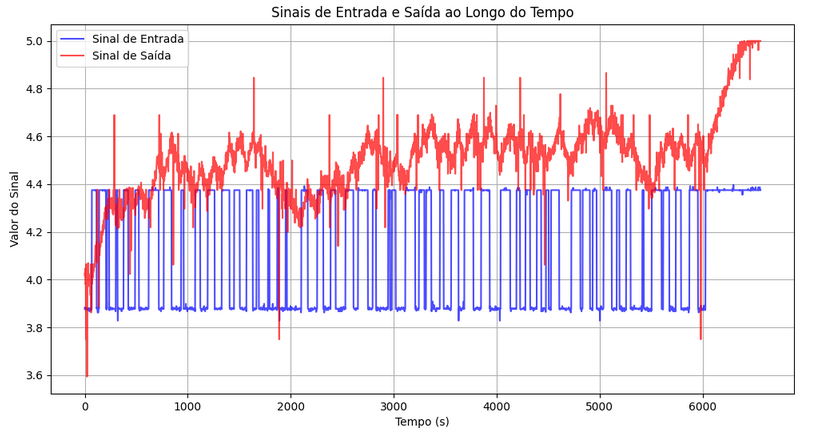
\includegraphics[width=0.8\textwidth]{12_1_1.png}
\caption{Sinais de entrada e saída ao longo do tempo. A entrada apresenta comportamento binário pseudoaleatório, enquanto a saída é mais suave devido à dinâmica do sistema.}
\label{fig:signals}
\end{figure}

\begin{figure}[h]
\centering
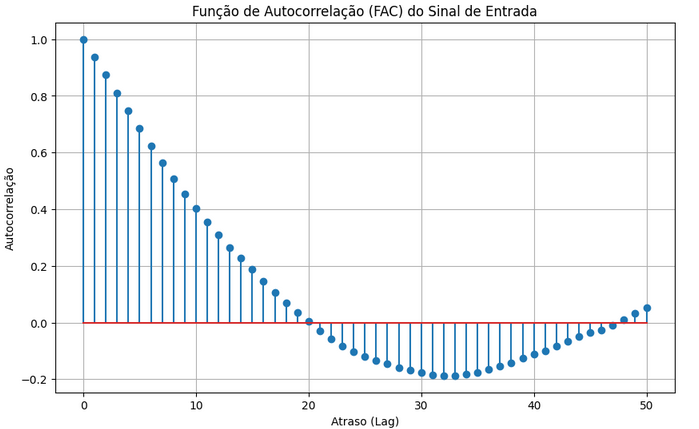
\includegraphics[width=0.8\textwidth]{12_1_2.png}
\caption{Função de autocorrelação (FAC) do sinal de entrada. Os altos valores iniciais indicam padrões determinísticos no sinal pseudoaleatório.}
\label{fig:autocorr}
\end{figure}

\newpage

\subsection{Discussão}

A função de autocorrelação mostra que ...

\subsection{Conclusão}
O sinal de entrada apresenta ...


\section{Exercício 12.2}

\subsection{Objetivo}
O objetivo deste exercício é ...

\subsection{Metodologia}

Os seguintes passos foram seguidos para resolver o problema...

\subsection{Resultados}

\begin{figure}[h]
\centering
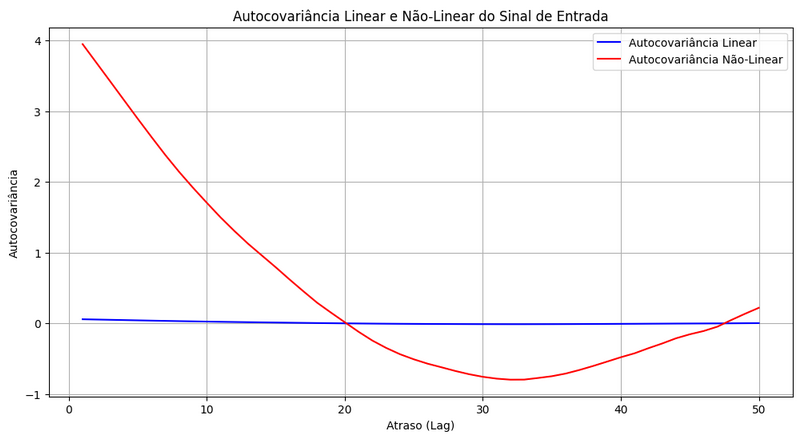
\includegraphics[width=0.8\textwidth]{12_2.png}
\caption{Autocovariância Linear e Não-Linear do Sinal de Entrada.}
\label{fig:autocovariance}
\end{figure}

\begin{itemize}
\item \textbf{Taxa de Decimação ($\Delta$):} 32.
\item \textbf{Número de observações no sinal decimado:} 101.
\item \textbf{Comprimento médio dos patamares mais curtos:} 2,37 observações.
\end{itemize}

\subsection{Discussão}

Os resultados indicam que ...

\subsection{Conclusão}

O sinal foi decimado utilizando...

\section{Exercício 12.3}

\subsection{Objetivo}
O objetivo deste exercício é...

\subsection{Metodologia}

Os seguintes passos foram realizados... 

\subsection{Resultados}

Os principais resultados obtidos foram:

\begin{itemize}
\item \textbf{Dimensão da matriz $Z$:} $96 \times 9$.
\item \textbf{Dimensão da matriz $Z^T Z$:} $9 \times 9$.
\item \textbf{Autovalores de $Z^T Z$:}
\begin{align*}
{-2.61 \times 10^{-15}, 2.43 \times 10^{-15}, 0.202, 0.792, 2.82, 22.78, 28.35, 44.17, 46.99}.
\end{align*}
\item \textbf{Multiplicidade do menor autovalor:} $2$.
\end{itemize}

\begin{figure}[h]
\centering
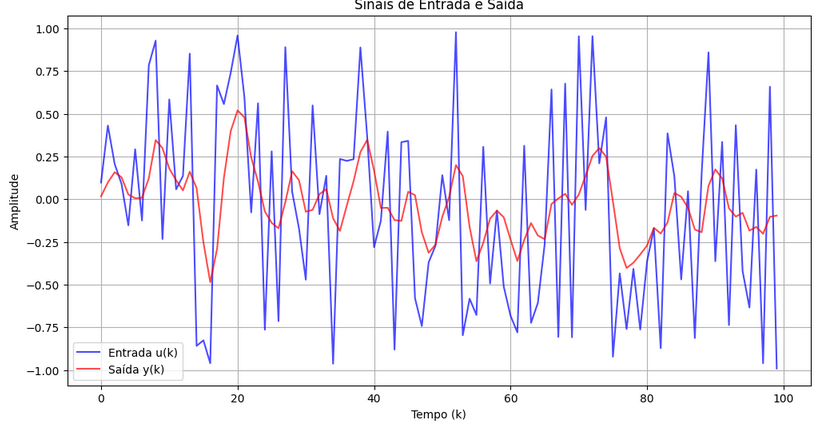
\includegraphics[width=0.8\textwidth]{12_3.png}
\caption{Sinais de Entrada e Saída.}
\label{fig:Sinais de Entrada e Saída}
\end{figure}

\subsection{Discussão}

A matriz de covariância $Z^T Z$ apresentou ...

\subsection{Conclusão}

O exercício demonstrou ...


%========================= Referências =========================================

\bibliography{references}

\end{document}